% Drawing 156-8/02-2 -- folder 156-8, batch 02, archive page 26 (PDF page 27).
% Transcription: dans la marge gauche, deux triangles : dans le premier un arc de cercle s'appuie sur la base, dans le second un arc joint deux sommets de la base.
% Kind: two triangles with arcs. Method 2 (schematic redraw from the facsimile). Status: ok.
% Notes: Left margin: in the first triangle an arc stands on the base between two points of it; in the second an arc joins the two base vertices. The legends under them (X << Y, ...) are text of the transcription.
% Coordinates: 1 unit = 1 mm = 1/100 of the crop width (bbox in page fractions: [0.1, 0.28, 0.27, 0.39]).
% Redrawn by Claude (claude-opus-5-5), issue #73 pilot, 2026-11-07; not checked by a human; not compiled (no TeX in the session).
% Rights: reproduces part of the work -- behind RENDER_TRANSCRIPTS, never published by itself.
\documentclass[tikz,border=3pt]{standalone}
\usepackage{amsmath,amssymb}
\usetikzlibrary{patterns,arrows.meta}
\tikzset{pencil/.style={black!45}, struck/.style={black!35}, mark/.style={circle,draw,inner sep=1.3pt}, pt/.style={circle,fill,inner sep=0.9pt}, opt/.style={circle,draw,fill=white,inner sep=1.1pt}}
\begin{document}
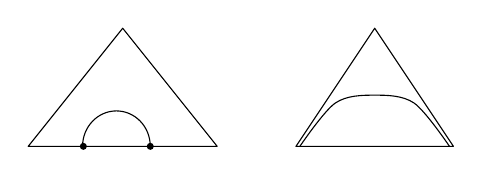
\begin{tikzpicture}[x=1mm,y=1mm,line cap=round,line join=round,font=\scriptsize]
\draw (33,-41) -- (21,-56) -- (45,-56) -- cycle;
\draw (36.5,-56) arc[start angle=0, end angle=180, x radius=4.3, y radius=4.5];
\node[pt] at (28,-56) {};
\node[pt] at (36.5,-56) {};
\draw (65,-41) -- (55,-56) -- (75,-56) -- cycle;
\draw plot[smooth, tension=0.55] coordinates {(55.5,-56) (60,-50.5) (65,-49.5) (70,-50.5) (74.5,-56)};
\end{tikzpicture}
\end{document}
